\documentclass[11pt]{article}

% ---------- Packages ----------
\usepackage[margin=1in]{geometry}
\usepackage{graphicx}
\usepackage{float}
\usepackage{booktabs}
\usepackage{tabularx}
\usepackage{array}
\usepackage{amsmath,amssymb,mathtools}
\usepackage{siunitx}
\usepackage{enumitem}
\usepackage{xcolor}
\usepackage{fancyhdr}
\usepackage{titlesec}
\usepackage{titling}
\usepackage{url}
\usepackage{microtype}
\usepackage{caption}
\usepackage{hyperref}

\setlength{\parskip}{0.5em}
\setlength{\parindent}{0pt}
\setcounter{tocdepth}{2}

% ---------- Custom commands ----------
\newcommand{\ProjectTitle}{Progressive AI on Multi-modality Tests for Differential Diagnosis of Early and Prevalent Neurological Disorders of Parkinson's Patients}
\newcommand{\Sponsor}{Michael J. Fox Foundation; Peter O'Donnel Foundation; Jim Holland (Backcountry); Michael \& Connie Rasor}
\newcommand{\ProjectPI}{Chandrajit Bajaj\\http://www.cs.utexas.edu/~bajaj}
\newcommand{\Institution}{Computer Visualization Center//http://}
\newcommand{\ReportDate}{October 2025}
%\newcommand{\Version}{v1.0}
\newcommand{\ProjectID}{[Internal Project ID]}

\definecolor{todo}{RGB}{180,0,0}
\definecolor{placeholder}{RGB}{120,120,120}
\newcommand{\TODO}[1]{\textcolor{todo}{\textbf{TODO:}~#1}}
\newcommand{\placeholder}[1]{\textcolor{placeholder}{\emph{[#1]}}}

% ---------- Hyperref ----------
\hypersetup{
    colorlinks=true,
    linkcolor=blue!60!black,
    citecolor=blue!60!black,
    urlcolor=blue!60!black,
    pdfauthor={\ProjectPI},
    pdftitle={\ProjectTitle},
    pdfsubject={Progress-to-Date Technical Report}
}

% ---------- Header / Footer ----------
\pagestyle{fancy}
\fancyhf{}
\lhead{\ProjectTitle}
% \rhead{\Sponsor}  % this long string causes overlap
\rhead{\textsc{Funding Partners}}  % replace with a shorter label
\cfoot{\thepage}

% ---------- Title ----------
\pretitle{\begin{center}\LARGE\bfseries}
\posttitle{\par\end{center}\vspace{0.5em}}
\preauthor{\begin{center}}
\postauthor{\par\end{center}}
\predate{\begin{center}}
\postdate{\par\end{center}}

\title{Progress-to-Date Technical Report}
\author{\ProjectPI\\ \Institution}
\date{\ReportDate}

% ---------- Section formatting ----------
\titleformat{\section}{\large\bfseries}{\thesection}{0.5em}{}
\titleformat{\subsection}{\normalsize\bfseries}{\thesubsection}{0.5em}{}
\titleformat{\subsubsection}{\normalsize\itshape}{\thesubsubsection}{0.5em}{}

% ---------- Useful column types ----------
\newcolumntype{Y}{>{\raggedright\arraybackslash}X}
\newcolumntype{Z}{>{\centering\arraybackslash}X}

% ---------- Document ----------
\begin{document}

\begin{titlepage}
    \centering
    {\Large \textsc{Our Funding Partners}}\par\vspace{0.6em}
    \begin{tabular}{@{}l@{}}
        Michael J.\ Fox Foundation (Grant MJFF--022670) \\
        Oden Institute for Computational Engineering and Sciences \\
        Jim Holland (Backcountry) \\
        Michael \& Connie Rasor \\
    \end{tabular}\par
    \vspace{1.8em}

    {\huge \textbf{\ProjectTitle} \par}
    \vspace{0.5em}
    {\Large Final Report}\par
    \vspace{1em}
    {\large \ReportDate}\par
    \vspace{1em}

    {\Large \textbf{Principal Investigator}}\par
    {\large Professor \ProjectPI}\par
    \vspace{1em}

    {\Large \textbf{Research Team}}\par
    {\normalsize
    Aaron Dominick \quad Ashwin Vinod \quad Aditya Sai \quad Aparna Dev \quad Shubham Bhardwaj \\
    Jasmine Khalil \quad Priyanshi Yadav \quad Ojas Phirke \quad Thribhuvan Rapolu \quad Aditya Rajnarayan \quad Harsh Tirhekar}\par
    \vspace{1em}

    {\Large \textbf{Clinical Collaborator}}\par
    {\normalsize
     Dr. Conor Fearon\\MD, Phd, Neurologist at Mater Misericordiae University Hospital, Dublin, Ireland\\Dr. Barbara Marebwa, \\Senior Scientist, Manager at the Michael J. Fox Foundation}\par
    \vspace{1em}
    

    {\Large \textbf{Original Proposal Project Title (MJFF Grant)}}\par
    {\normalsize ``Actionable Intelligence of Imaging Biomarkers Discovery Towards Early Diagnosis and Effective Prognosis for Parkinson’s Disease''}\par
    \vspace{1em}

    \begin{tabular}{@{}ll@{}}
        Contract / Grant: & MJFF--022670 \\
        Funding Source: & Michael J.\ Fox Foundation \\
        Period: & November 1, 2022 -- October 31, 2024 \\
        Total Award: & \$300{,}132 (Direct and Indirect) \\
        %In-Kind Support: & Jim Holland -- Backcountry (\$200{,}000) \\
        Distribution: & \textbf{For Funding Partners Only}
    \end{tabular}
    \vfill

    {\footnotesize
    This work is conducted under the Michael J.\ Fox Foundation grant MJFF--022670 and in-kind 
    collaboration with the Oden Institute for Computational Engineering and Sciences at the University of 
    Texas at Austin. The project integrates clinical, imaging, genetic, and biospecimen data from PPMI 
    and partner datasets to advance early diagnostic and prognostic modeling of Parkinson’s disease 
    through multi-agent actionable machine learning systems.}

\end{titlepage}


\newpage
% \tableofcontents
% \newpage
% \listoftables
% \listoffigures
% \newpage

\section{Executive Summary}
\label{sec:exec-summary}

This final report summarizes the progress and ongoing work in our Progressive AI program with specific aims to achieve
differential diagnosis of  specific neurological disorders affecting patients with possible Parkinson's diesease. We build  actionable, multi-modal data agents for generatively subgrouping patients into multi-symptomatic latent subspaces with varying  Parkinson’s disease (PD)  severity.
The learned objectives are to fuse clinical scales, DaT--SPECT and structural/diffusion MRI, genetics/biospecimens, and wearable time series to enable robust early detection, identify imaging and behavioral patterns that differentiate phenotypic subtypes, and support longitudinal, quantitative tracking of disease state. The framing remains aligned with the original aims: curate multi-modal cohorts; train modality-specific \emph{actionable machine learning} agents coordinated by a master agent; discover radiomic and kinematic signatures; and learn extended-Kalman co-regionalized progression models.

We have organized and harmonized core PPMI assets (MDS--UPDRS, UPSIT, REM-sleep and other non-motor scales; DaTscan SPECT; T1 and diffusion MRI; SNP/WGS) and integrated additional patient data (blood/CSF markers and MRI) provided via philanthropic support. These assets underpin the cross-validation and testing workflows for both modeling and clinician-facing evaluation.

Two pillars structure the body of this report. The first, \emph{multi-modal agents (silos)}, comprises domain-specific pipelines for imaging, diffusion--clinical co-clustering, gait/arm-swing analytics, and mechanism inference \cite{dominick2025brain,vinod2025compositional,khalil2025multimodal,tirhekar2025comprehensive}. The second, \emph{workflows}, implements (i) generative latent-space construction using scalable robust Bayesian co-clustering to align imaging and clinical measures \cite{vinod2025scalable,vinod2025compositional}; and (ii) a clinician’s workflow that operationalizes these latent inferences through interactive visualization and case-review tools (\url{https://cvc-lab.github.io/parkinson-viz/}).

Interim findings show that integrating diffusion metrics with clinical scales yields subtypes that track severity and cognitive decline; that DaT--SPECT and T1-derived region-wise features can differentiate CSFSAA-positive and CSFSAA-negative Parkinsonisms; and that wearable-derived gait and arm-swing metrics predict and phenotype CSF {$\alpha$}-synuclein status, offering a non-invasive complement to imaging and biospecimens \cite{dominick2025brain,vinod2025compositional,khalil2025multimodal}. A mechanism-inference analysis provides code-backed claims connecting these markers to hypothesized biological pathways, enabling traceable reasoning across modalities \cite{tirhekar2025comprehensive}.

The core agent infrastructure and imaging pipelines are implemented; diffusion--clinical co-clustering and gait/arm-swing phenotyping are trained on harmonized cohorts; and clinician-facing interfaces are prototyped. Near-term priorities are prospective validation on held-out sites/cycles, calibration and drift audits across devices and acquisition protocols, subgroup fairness reporting, and formalization of SOPs for case review and longitudinal follow-up.


\textbf{Overview.} The body of this report is organized around the program’s two pillars—\emph{multi‑modal agents} and \emph{clinical workflows}—and four domain contributions. First, \emph{Multi‑modal Agents}: we have implemented master–drone AML agents that perform rank‑ordered information search and scoring within each modality, using controlled neural ODE encoders/decoders with Kalman filtering and iLQG‑based policy updates under a POMDP formulation. We also developed a sample‑efficient multi‑agent reinforcement learning variant for coordinated cross‑modal querying. These implementations operationalize the “actionable intelligence” design proposed to the sponsor and now serve as shared infrastructure for all downstream studies.

Second, \emph{DaTscan/T1 imaging pipeline}: an automated pipeline ingests DaT--SPECT and T1‑MRI, performs atlas‑constrained segmentation, extracts region‑wise volumetric and dopaminergic features, ranks them for stability and discriminability, and feeds them to downstream classifiers. This pipeline and its figure are documented in Dominick \& Bajaj (2025), which we reference in Part~2 as the canonical description of the imaging‑biomarker workflow.

Third, \emph{DTI+clinical co‑clustering}: a compositional Bayesian co‑clustering model integrates diffusion biomarkers with clinical measures to discover severity‑aligned subgroups while retaining mechanistic interpretability. The approach (Vinod \& Bajaj, 2025) is trained with a compositional ELBO and mutual‑information alignment across views, and its scalable variant (Vinod \& Bajaj, 2025, arXiv:2504.04079) is used to construct generative latent spaces per modality, forming \textbf{Workflow~1}.

Fourth, \emph{Gait/arm‑swing and $\alpha$‑syn phenotyping}: a multimodal learner predicts and phenotypes CSF $\alpha$‑syn status using wearable‑derived gait/arm‑swing metrics with cognition/demographics (Khalil \& Bajaj, 2025), offering a non‑invasive complement to imaging and biospecimens for stratification.

Complementing these, a \emph{mechanism‑inference} analysis (Tirhekar \& Yadav, 2025) systematically enumerates and tests mechanistic claims, providing traceable code evidence and interpretations that connect observed biomarkers to putative biological pathways and risks. This analysis framework is integrated into the report’s Part~2 to contextualize the discovered subtypes and signatures.

\textbf{Clinical translation and workflows.} In \textbf{Workflow~2}, we document the clinician’s path through our interactive tools and the demonstration: per‑patient review of movement quality, symmetry, and gait cycles alongside UPDRS; cross‑visit overlays; and cohort views for differential diagnosis and monitoring. Together with Workflow~1’s generative latent spaces, this provides an end‑to‑end path from raw multi‑modal signals to decision support.

\textbf{Status and next steps.} The core agent infrastructure and imaging pipelines are implemented; DTI+clinical co‑clustering and gait/arm‑swing phenotyping are trained on harmonized cohorts; and clinician‑facing interfaces are prototyped. Near‑term priorities, consistent with the proposal, are prospective validation on held‑out sites/cycles, calibration and drift audits across devices and acquisition protocols, subgroup fairness reporting, and formalization of SOPs for case review and longitudinal follow‑up. 



\section{Methodology}
\label{sec:methodology}

\subsection{Workflows}

The program operationalizes two complementary workflows that unify multi-modal inference with clinical interpretation. 

\subsubsection{Workflow~1: Generative latent-space modeling of multimodal data}
We construct harmonized latent representations from imaging, diffusion, and clinical modalities using scalable, robust Bayesian co-clustering. The framework jointly embeds subject-level matrices of region-specific imaging biomarkers (DTI, DaT, and T1 MRI) and clinical scores (UPDRS, MoCA, UPSIT, SCOPA-AUT), with Gaussian-mixture priors on both patient and feature encoders and a joint variational ELBO. Mutual-information and compositional KL regularizations enforce alignment between clinical and imaging subspaces, yielding biologically interpretable clusters rather than purely statistical partitions. This architecture reveals subtypes consistent with PD severity gradations and cognitive decline; a scalable implementation supports multi-site training and evaluation \cite{vinod2025compositional,vinod2025scalable}.

\subsubsection{Workflow~2: Clinician-centric decision and visualization pipeline}
A deployment-oriented pipeline ingests outputs from Workflow~1 and presents patient-specific movement, gait, and cognitive data for interactive use. Clinicians can visualize motion asymmetry, arm-swing coordination, and gait trajectories alongside UPDRS-III motor subscores, compare performance across visits, and identify deviations from subtype-level baselines. Cohort overlays and timeline navigation operationalize latent-space inferences for case review and longitudinal monitoring (\url{https://cvc-lab.github.io/parkinson-viz/}).

\subsection{Multi-Modal Agents (silos)}

The \emph{silos} are modality-focused pipelines that extract, align, and interpret complementary information; each functions as a specialized agent within the \emph{Progressive AI} architecture.

\subsubsection{Imaging silo: DaTscan--T1 feature extraction and ranking}
This silo extracts region-wise structural (T1-MRI) and dopaminergic (DaT-SPECT) biomarkers and ranks them by discriminability and stability for separating CSFSAA$^+$ vs.\ CSFSAA$^-$ Parkinsonisms, following the pipeline in Fig.~\ref{fig:datscan-pipeline} \cite{dominick2025brain}. T1-MRI scans are segmented into 108 Desikan--Killiany--Tourville ROIs with a SegFormer model trained on Mindboggle-101; DaT-SPECT is coregistered to MNI and summarized within each ROI via SBR-derived Gaussian‑process moments (mean, SD, skewness, kurtosis). The resulting imaging matrix (volumes + DaT features) is used for supervised ranking and downstream subgrouping (Fig.~\ref{fig:imaging-workflow}).

\textbf{Results.} Imaging alone provides fair discrimination of CSFSAA status ($\mathrm{AUC}=0.7031\pm0.078$), with larger cuneus volume and smaller pars opercularis and putamen volumes characteristic of CSFSAA$^-$ patients. Non‑imaging anchors show UPSIT ($0.7608\pm0.084$) and di‑22{:}6‑BMP ($0.8553\pm0.078$) as strong single‑modality predictors; fusing imaging with clinical/biological features yields excellent performance ($0.9318\pm0.036$). Co‑clustering sharpened stratification when imaging was included, revealing two SAA‑low subgroups (0\% and 4\% CSFSAA$^+$; $p<10^{-3}$ and $p<10^{-4}$) and one SAA‑high subgroup (73.8\%; $p<10^{-3}$). Salient imaging drivers concentrated in cuneus volume, paracentral DaT‑SPECT skewness, and pallidal DaT‑SPECT skewness (Fig.~\ref{fig:imaging-cocluster}). See \cite{dominick2025brain} for cohort details, preprocessing, and full analytics.

\begin{figure}[h!]
    \centering
    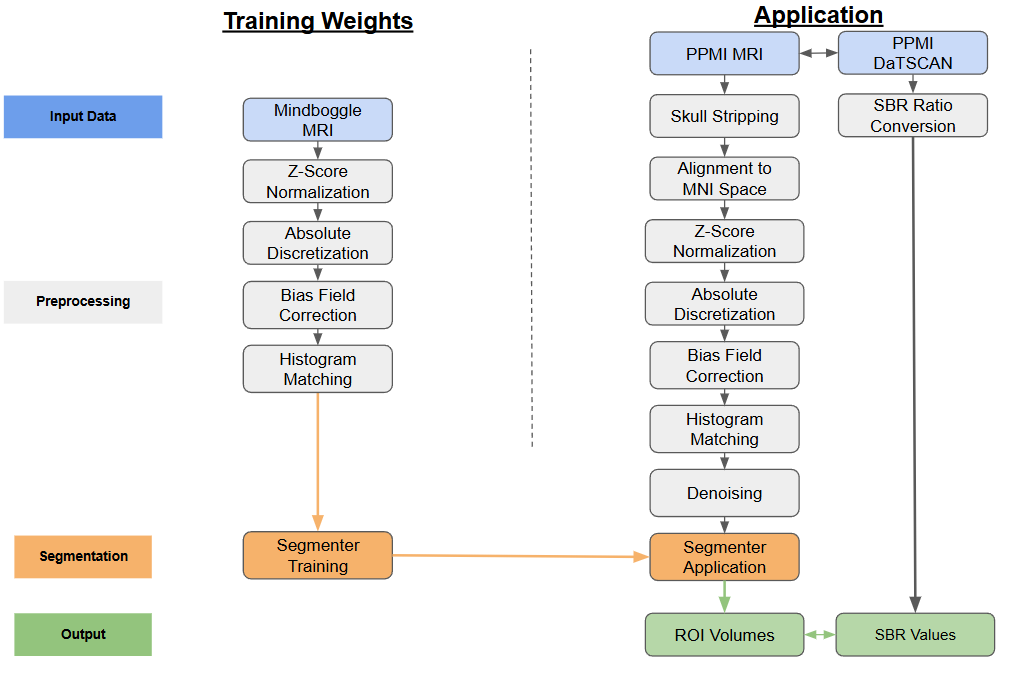
\includegraphics[width=0.85\linewidth]{figures/SegmentationPreprocessing.png}
    \caption{\textbf{Imaging feature extraction pipeline.} Mindboggle‑101–trained SegFormer with harmonized preprocessing yields 108 ROI masks on PPMI MRIs; ROI volumes and DaT‑SPECT features (SBR‑based moments) are computed. Source: \cite{dominick2025brain}, cf.\ Fig.~1, p.~5.}
    \label{fig:datscan-pipeline}
\end{figure}

\begin{figure}[h!]
    \centering
    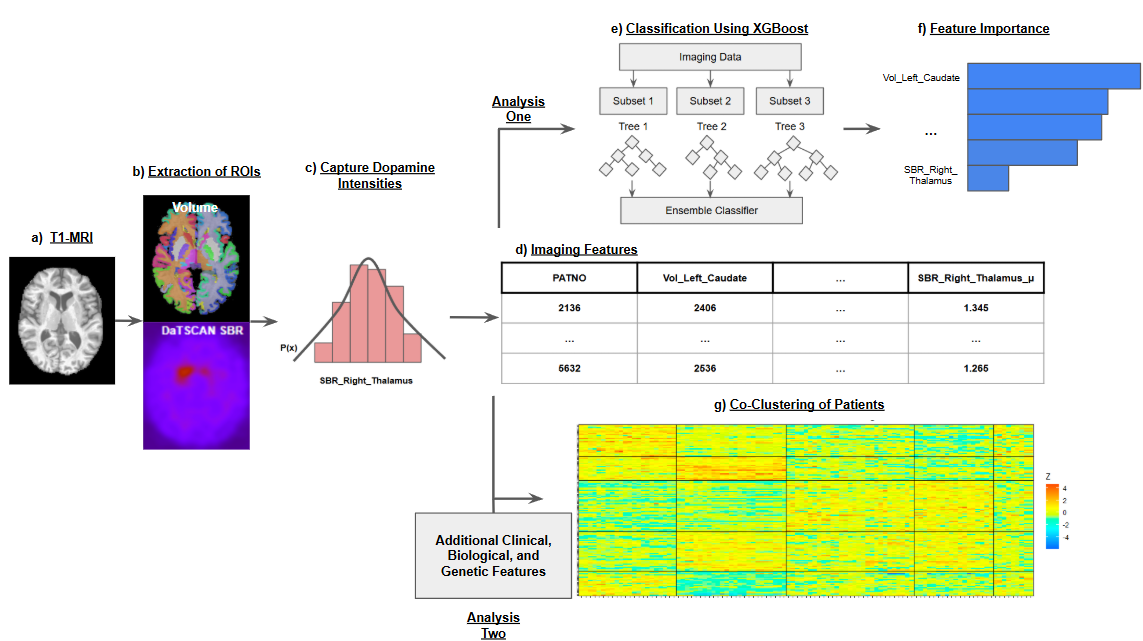
\includegraphics[width=\linewidth]{figures/NewProcess.png}
    \caption{\textbf{Analysis workflow.} (a–d) ROI extraction and DaT‑SPECT modeling; (e–f) XGBoost classification and feature ranking; (g) co‑clustering with selected imaging + clinical/biological/genetic features. Source: \cite{dominick2025brain}, cf.\ Fig.~2, p.~8.}
    \label{fig:imaging-workflow}
\end{figure}

\begin{figure}[h!]
    \centering
    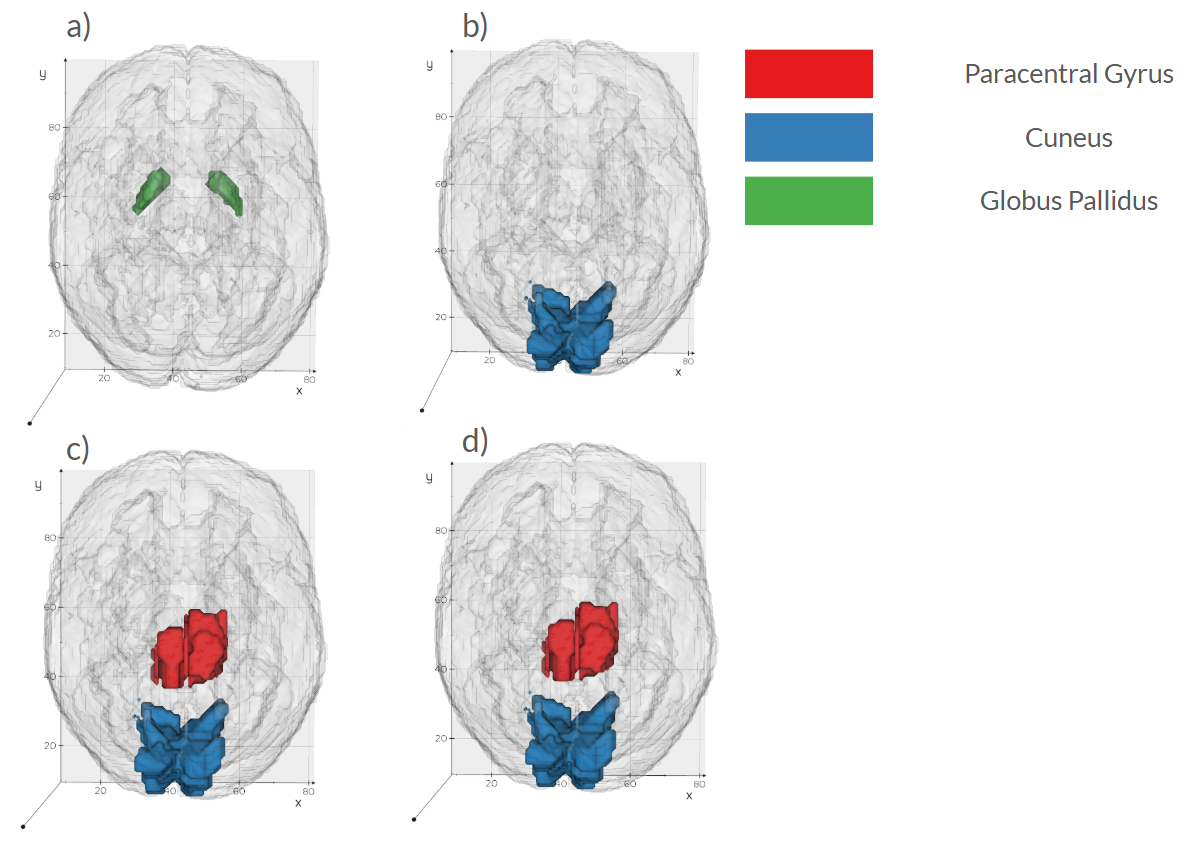
\includegraphics[width=\linewidth]{figures/CoclusterImages.png}
    \caption{\textbf{Representative subgroup‑specific imaging markers.} (a) globus pallidus DaT‑SPECT skewness; (b) cuneus volume; (c–d) cuneus volume with paracentral DaT‑SPECT skewness---features that drive SAA‑low/high subgroup separation. Source: \cite{dominick2025brain}, cf.\ Fig.~23, p.~40.}
    \label{fig:imaging-cocluster}
\end{figure}

\subsubsection{Diffusion--clinical silo: Bayesian co-clustering}
Free-water–corrected fractional anisotropy and mean diffusivity metrics across subcortical regions are fused with UPDRS and MoCA scores into a joint feature matrix. A compositional Bayesian co-clustering model learns paired encoders for patients and features with information alignment between diffusion asymmetries and clinical outcomes, identifying three dominant patient clusters along a clear severity gradient \cite{vinod2025compositional}.

The pipeline outputs a single feature table in which each row represents an ROI and each column represents a modality-specific metric (volume, SBR, FA, MD, or free-water fraction).  Because every preprocessing stage is executed within a harmonised coordinate system and capped by a dedicated quality-control step, the resulting feature set is internally consistent and suitable for cross-sectional or longitudinal modelling of Parkinson’s disease progression. Our Multi modal extraction pipeline is shown in Fig. \ref{fig:mm_overview} .
\begin{figure*}[htbp]
  \centering
  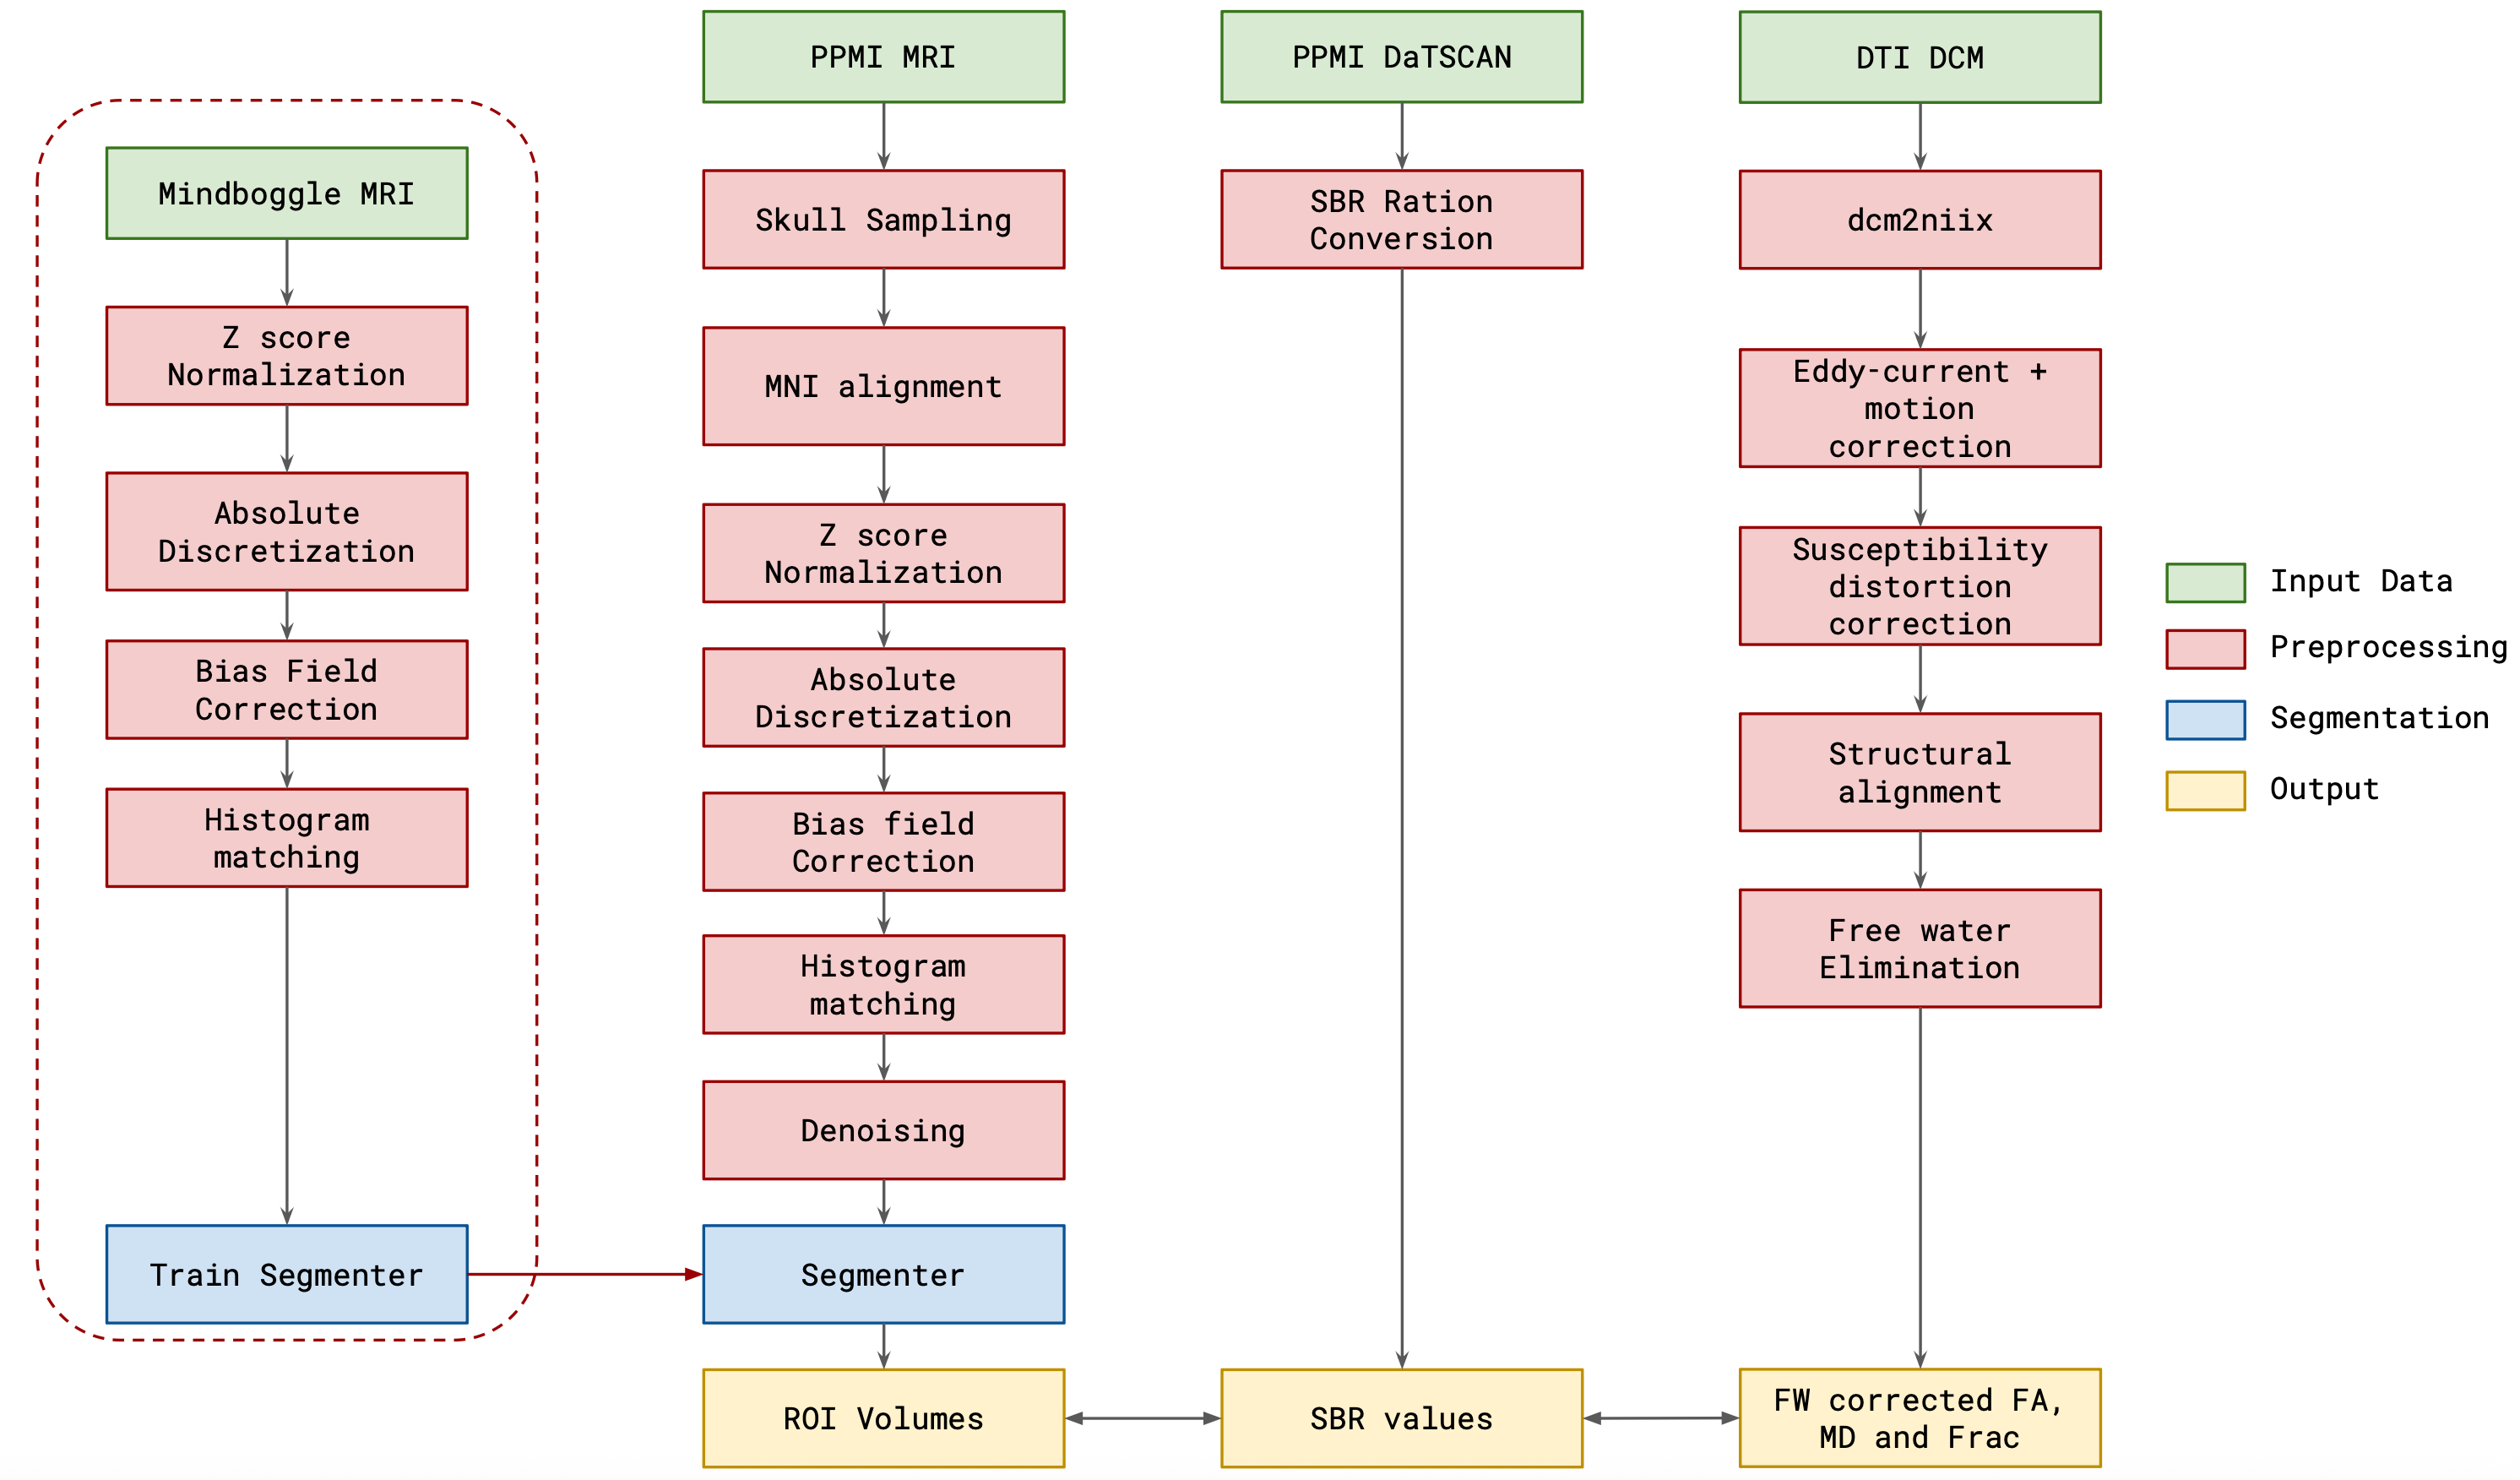
\includegraphics[width=\textwidth]{figures/DTI_fwe.png}
  \caption{Multimodal Feature extraction pipeline}
  \label{fig:mm_overview}
\end{figure*}

Our co-clustering framework a described in Fig. \ref{fig:cc_pd_pipeline} employs \text{dual variational autoencoders} for instances and features, each regularized by \text{Gaussian mixture priors} that induce soft cluster assignments in their respective latent spaces. A \text{joint latent variable} captures cell-level (patient-feature) interactions via a \textit{compositional Evidence Lower Bound (ELBO)}, augmented with double reparameterized gradients (DREGs) to enhance signal-to-noise separation and mitigate posterior collapse. Mutual information based cross-losses enforce alignment between clinical and neuroimaging manifolds, ensuring coherent row-column partitions even under noise or missing data. 
 We use this \textit{Scalable Robust Variational Co-Clustering (SRVCC)} framework to integrates DaTSCAN, volumetric MRI, and diffusion measures with clinical scores to reveal interpretable Parkinson’s disease subtypes spanning mild, moderate, and advanced stages.

 \begin{figure*}[htbp]
  \centering
  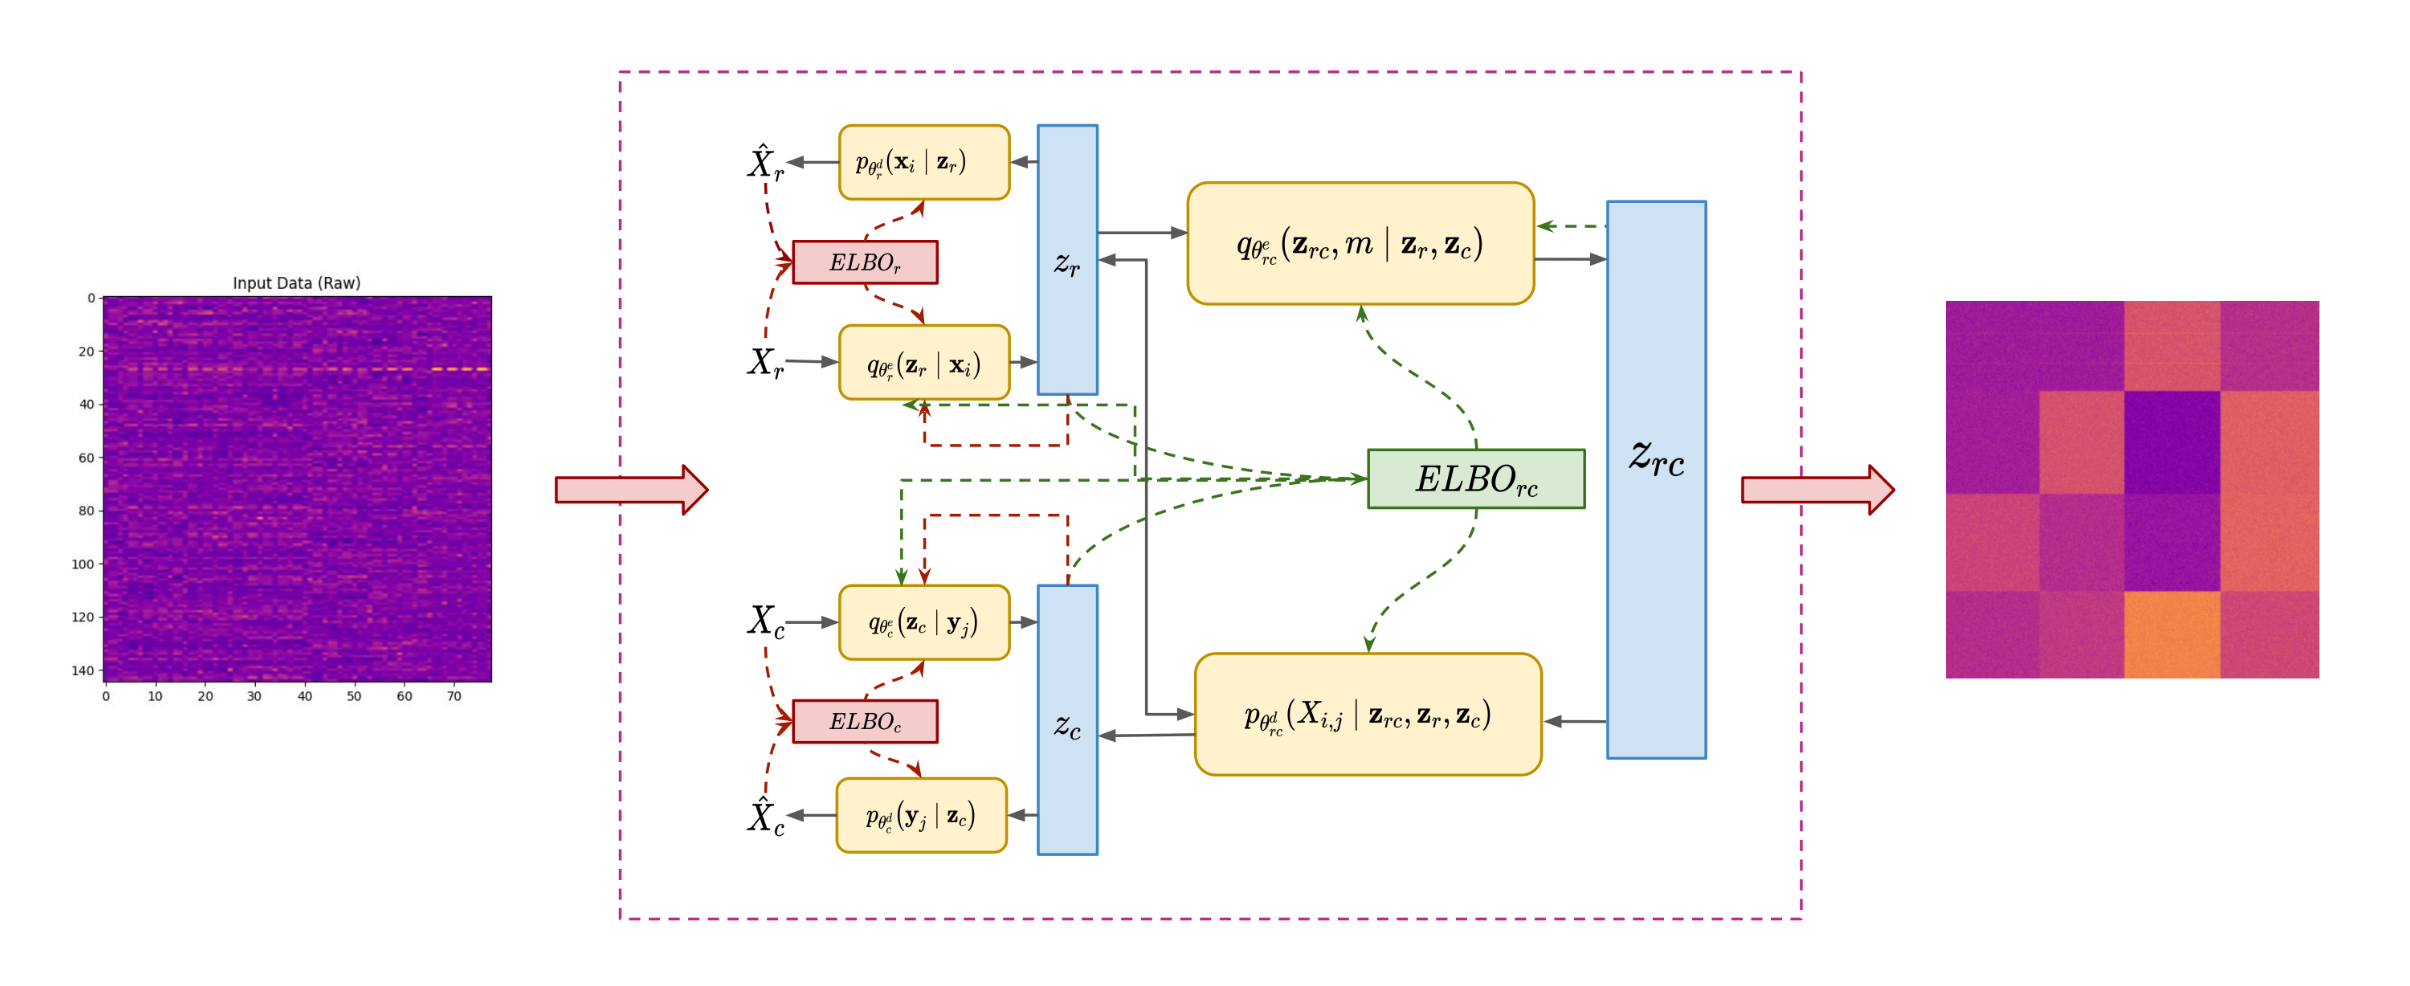
\includegraphics[width=\textwidth]{figures/cc_pd_pipeline.png}
  \caption{The multi-modal feature-extraction pipeline produces a pre-processed data matrix, which is then passed to our Scalable Bayesian Co-clustering framework. The framework reorganizes the matrix into a checkerboard pattern, re-
vealing coherent, clustered patient groups.}
  \label{fig:cc_pd_pipeline}
\end{figure*}
 
\subsubsection{Wearable–cognitive silo: gait and arm-swing phenotyping}
This work utilizes wearable sensor data to characterize gait and upper-limb movement during three standardized mobility assessments from the Parkinson’s Progression Markers Initiative (PPMI) Gait and Arm Swing Substudy. These tasks capture complementary aspects of motor function relevant to early Parkinson’s disease (PD) detection, including walking stability, cognitive–motor interaction, and turning control.


\textbf{Study Goals.}
The objective of this component is to establish a scalable, sensor-based framework for quantifying motor biomarkers associated with PD pathology. We aim to determine whether features derived from wearable sensors can contribute to the non-invasive prediction of CSF $\alpha$-synuclein seed amplification assay (CSFSAA) status, a biological benchmark of PD.

\textbf{Cohorts and Data Modalities.}
To contextualize the data collection process, Fig. \ref{fig:gaitassessments} illustrates the sequence of steps during the three main gait assessments. We analyzed baseline data from 84 participants in PPMI, each with confirmed CSFSAA status. The following modalities were included:
\begin{itemize}
    \item Wearable-derived gait and arm-swing features: Over 50 metrics extracted from IMU sensors on the lumbar spine and both wrists during standardized mobility tasks (Timed Up and Go, Usual Walk, Dual-Task Walk, and Postural Sway).
    \item Clinical and cognitive assessments: MDS-UPDRS, HVLT-Retention, Epworth Sleepiness Scale, and related cognitive-behavioral measures.
    \item Demographics and biomarker data: Age, sex, and disease duration.
\end{itemize}

As shown in Figure \ref{fig:gaitassessments}, gait was recorded using three APDM Opal sensors placed on the lower back and both wrists. Each sensor captured tri-axial accelerometer and gyroscope data, which were used to derive over 50 gait and arm swing features quantifying amplitude, timing, asymmetry, and coordination.

\begin{figure}[h!]
    \centering
    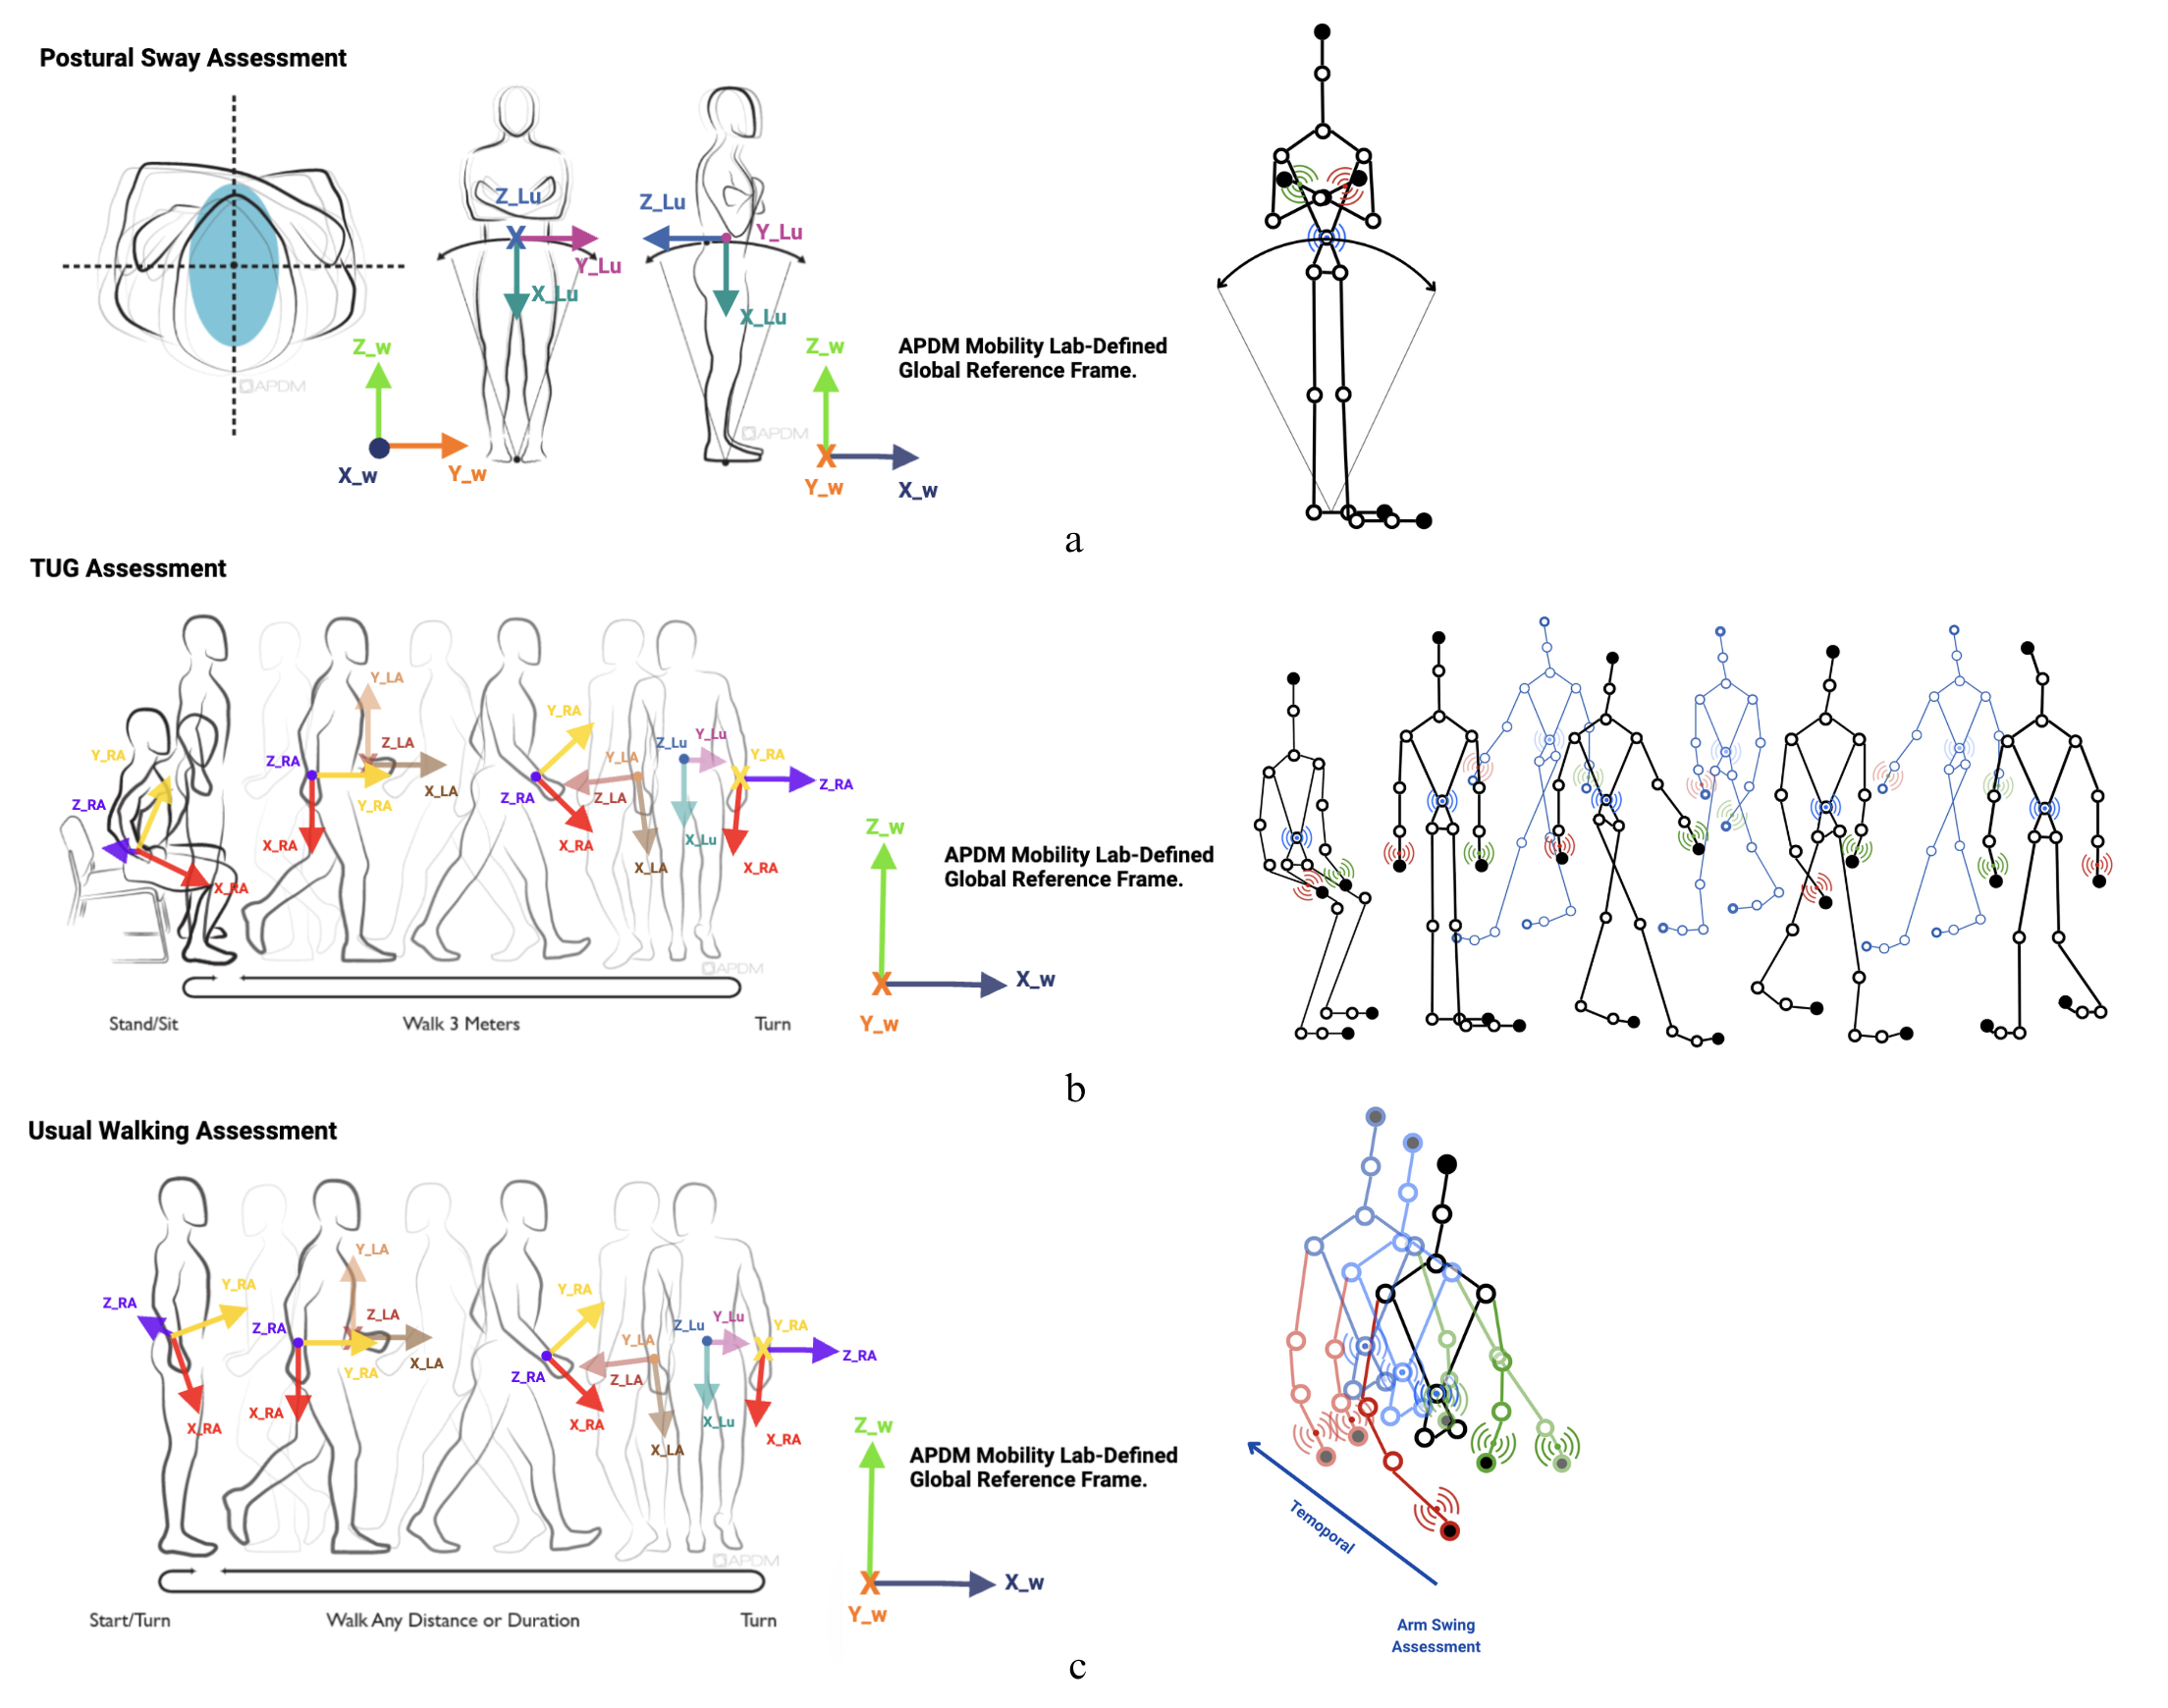
\includegraphics[width=1\linewidth]{figures/gaitassessments.png}
    \caption{Visual presentation of the steps taken during the three main structured assessments. (a) Postural Sway Assessment. (b) TUG Assessment. (c) Usual Walking Assessment. Each part includes the local coordinate system of the IMU Opal sensor, the world coordinate system, and a spatiotemporal skeletal model capturing how localized movement at one joint or limb propagates through and affects the kinematics of the entire body.}
    \label{fig:gaitassessments}
\end{figure}

\textbf{Key Findings.}
\begin{itemize}
    \item \textbf{Predictive modeling:} Histogram-based Gradient Boosting achieved strong classification accuracy for CSFSAA positivity (AUC = 0.931 $\pm$ 0.065) using multimodal features.
    \item \textbf{Feature importance:} SHAP analysis identified memory retention (HVLT-Retention), daytime sleepiness (Epworth Sleepiness Scale), and right arm jerk amplitude as key predictors.
    \item \textbf{Gait contribution:} Gait features alone were less discriminative (AUC = 0.58 $\pm$ 0.16) but improved performance when combined with other modalities.
    \item \textbf{Patient subgroups:} UMAP and spectral co-clustering revealed three phenotypes: motor-dominant, multimodal, and cognitive-dominant, each reflecting distinct $\alpha$-synuclein–related feature patterns.
\end{itemize}

This proof-of-concept study supports the feasibility of using non-invasive and multimodal data to approximate CSFSAA status and identify biologically coherent PD subtypes. Although limited by sample size and cross-sectional design, the framework establishes a foundation for scalable biomarker discovery and early phenotyping. Full methodological details are provided in \cite{khalil2025multimodal}.


% \subsubsection{Mechanism-inference silo}
% A complementary analysis enumerates mechanistic claims with code evidence, linking imaging and wearable-derived markers to putative {$\alpha$}-synuclein pathways, dopaminergic dysfunction, and neuroinflammation, thereby grounding empirical signatures in mechanism-centric hypotheses \cite{tirhekar2025comprehensive}.

\subsubsection{Mechanism-inference Silo}
A complementary analysis enumerates mechanistic claims with code evidence, linking imaging and wearable-derived markers to putative $\alpha$-synuclein pathways, dopaminergic dysfunction, and neuroinflammation, thereby grounding empirical signatures in mechanism-centric hypotheses \cite{tirhekar2025comprehensive}.

\textbf{Executive Summary and Research Objective} - 
The fundamental goal of this computational work is biological mechanism inference in Parkinson’s disease (PD). This represents a paradigm shift, moving beyond traditional symptom-based classification (e.g., classifying a patient as "tremor-dominant") to identify the specific underlying biological pathway dysfunctions, such as $LRRK2$ kinase hyperactivity, differential striatal vulnerability, or brainstem $\alpha$-synucleinopathy, that are the root cause of clinical presentations. This mechanism-based approach supports the future development of targeted, pathway-specific therapeutic interventions.
The analysis rigorously tested and verified 36 evidence-based claims across five major biological pathway categories implicated in PD pathogenesis:

\begin{itemize}[noitemsep, topsep=0.5em, partopsep=0pt, parsep=0pt]
    \item \textbf{Pathway 01: Dopaminergic Degeneration \& Motor Control:} Focused on the nigrostriatal tract and core motor symptoms.
    \item \textbf{Pathway 02: Genetic \& Molecular Mechanisms:} Focused on $LRRK2$ kinase dysfunction and $\alpha$-synuclein pathology.
    \item \textbf{Pathway 03: Cholinergic \& Cognitive Control:} Focused on olfaction (UPSIT) and REM sleep behavior disorder (RBD).
    \item \textbf{Pathway 06: Gait Dynamics \& Wearable Sensors:} Utilized objective IMU sensor metrics like arm swing asymmetry and Dual-Task Cost.
    \item \textbf{Pathway 08: Cross-Pathway Integration:} Synthesizing findings for multimodal patient characterization.
\end{itemize}

\textbf{Datasets and Patient Cohorts Used} - 
The study integrated large-scale multi-modal datasets from the Parkinson’s Progression Markers Initiative (PPMI) ($n=14,473$ total patients) and the LRRK2 Cohort Consortium ($n=2,958$ individuals). A crucial aspect of the research's Medical Research Ethics Framework was the maintenance of a strict \textbf{NO data imputation policy}; only actual measured values were analyzed, ensuring data integrity.
The specific sample sizes ($n$) for the key claims verified by this silo are transparently reported:

\begin{table}[H]
\centering
\caption{Key Data Modalities and Sample Sizes by Cohort \cite{tirhekar2025comprehensive}}
\label{tab:mechanism_cohorts_simple}
\small
\begin{tabularx}{\linewidth}{@{}Y Y Y@{}}
\toprule
\textbf{Cohort / Data Set} & \textbf{Data Modalities / Content Analyzed} & \textbf{Analysis Sample Size ($n$)} \\
\midrule
PPMI Core Motor & UPDRS-III Motor Assessment (Baseline) & 4,166 \\
PPMI Prodromal & Olfactory Function (UPSIT); RBD Assessment & 5,122 (Olfaction); 1,548 (RBD) \\
LRRK2 Consortium & $LRRK2$ G2019S Genetic Status & 2,958 \\
PPMI Wearables & Gait Dynamics (ASA, Dual-Task, TUG) & 172–178 \\
Biomarkers & urinary phospho-$LRRK2$; CSF SAA (RT-QuIC) & 884 (LRRK2); 145 (CSF SAA) \\
\bottomrule
\end{tabularx}
\end{table}

The computational methodology utilized a \textbf{Baseline-first strategy} to integrate the PPMI longitudinal study files, successfully preparing a merged baseline dataset of 4,775 unique patients across 388 features, thereby managing the challenge of longitudinal data explosion.

\textbf{Methodological Rigor and Innovations} - 
The identification of the 5 distinct motor phenotypes (Claim 1) utilized a cutting-edge unsupervised approach: the \textbf{Bayesian Gaussian Mixture Model (GMM) with a Dirichlet Process Prior}. This model allowed for the automatic selection of the optimal number of clusters based on the Bayesian Information Criterion (BIC). Crucially, the approach incorporated \textbf{Uncertainty Quantification}, allowing researchers to flag potential "mixed pathology" cases. The resulting clusters achieved a good level of separation, validated by a \textbf{Silhouette Score of 0.535}.

\textbf{Summary of Key Mechanism-Inference Findings (Tier 1 Discoveries)} - 
The analysis generated 36 claims, providing traceable statistical evidence and mechanistic interpretations. The Tier 1 and Tier 2 major discoveries include:

\begin{table}[H]
\centering
\caption{Tier 1 Discoveries Linking Pathways to Mechanisms \cite{tirhekar2025comprehensive}}
\label{tab:mechanism_tier1_findings}
\small
\begin{tabularx}{\linewidth}{@{}Y Y Y Y@{}}
\toprule
\textbf{Pathway} & \textbf{Finding (Claim \#)} & \textbf{Key Result / Statistic} & \textbf{Mechanism Inferred} \\
\midrule
Genetic (P02) & $LRRK2$ Genetic Risk (Claim 16) & 1.89$\times$ increased PD risk ($\chi^2=167.263, p<0.001$) & $LRRK2$ kinase hyperactivity accelerates dopaminergic degeneration \\
Dopaminergic (P01) & Motor Phenotype Heterogeneity (Claim 1) & 5 distinct subtypes identified (Silhouette $\mathbf{=0.535}$) & Reflects differential striatal vulnerability patterns \\
Cholinergic (P03) & Olfactory Dysfunction (Claim 21) & 50.2\% prevalence (UPSIT $< 25$) & Indicates early $\alpha$-synucleinopathy (Braak Stage 1-2 involvement) \\
Cholinergic (P03) & RBD Prevalence (Claim 22) & 37.5\% prevalence & Marker of brainstem $\alpha$-synucleinopathy (prodromal stage) \\
Gait (P06) & Dual-Task Cost (Claim 23/33) & 14.87\% gait speed degradation ($t=14.984, p<0.001$) & Cognitive-motor network failure and loss of gait automaticity \\
\bottomrule
\end{tabularx}
\end{table}

The correlation between objective gait speed and clinical motor severity (Spearman $r = -0.301, p = 0.000079, n=166$) further validates the use of wearable sensors, as both measures share a common biological substrate in dopaminergic circuit function. The identification of significant \textbf{Arm Swing Asymmetry} in 27.0\% of the analyzed cohort ($n=178$) confirms the utility of IMU sensors in capturing the lateralized nature of dopaminergic degeneration (Claim 30).

For detailed mathematical formulations of the Bayesian GMM and complete statistical log outputs for all 36 claims, readers are referred to Appendix F and Appendix B, respectively, of the comprehensive documentation \cite{tirhekar2025comprehensive}. These findings directly support the broader conclusions regarding stratified medicine and objective biomarker validation discussed in other sections of this report, such as the Wearable–cognitive silo.



\subsubsection{Integration}
Silo outputs feed a master inference layer that follows an actionable machine learning paradigm with controlled neural ODE encoders/decoders, extended Kalman filtering, and policy optimization for adaptive cross-modal coordination; this enables a unified, interpretable manifold supporting mechanistic insight and clinical translation (see also \cite{bajaj2025bayesian}).


% \section*{References}
\bibliographystyle{plain}
\bibliography{references}  

\appendix
\clearpage

\end{document}